\titleformat{\chapter}[display]   
{\normalfont\large\bfseries\centering}{\chaptertitlename\ \thechapter}{10pt}{\large}   
\titlespacing*{\chapter}{0pt}{-20pt}{25pt}
\chapter{Introduction}
\label{intro}
%\section{Effects of interaction on field-induced resonances in a confined Fermi liquid}
\section{Resonances in Many-Body Systems}
%MK changes
\subsection{Resonances in Nature and Technology}
%MK new paragraph
The phenomenon of the resonance is commonplace in nature.
It occurs in enormous variety of systems, microscopic and macroscopic, classical and quantum alike.  
When the frequency of external drive hits well defined set of values, the so called ``natural'' frequencies, its energy absorption becomes very large.
In a familiar example of a swing,  the easiest way to bring it into motion is to push it at time intervals matching the natural frequency of the swing.
The latter depends on the mass of a kid in the swing as well as the chain length.
In this and other cases the property of the system is revealed by its response to the external drive.
And the maximum response appears at frequencies that are characteristic to a system studied.
  
As a simplest model of the swing oscillations, consider a point particle of the mass $m$ attached to the string.
Let the displacement of the particle from its equilibrium position be $z$, 
The restoring force the string exerts on the particle is $ - K z$.
%MKone-dimentional 
%system (e.g. a string) 
Consider the vibrations of the particle under the influence of an external force, $F(t)$. 
The equation of motion of the spring end is %for such a system is %MK given by
\be\label{forcedosc}
\frac{d^2 z}{d t^2}+\frac{K}{m} z = \frac{F(t)}{m}\, .
\ee
%where, %$F(t)$ is the external force and $\omega$ is the natural frequency of free oscillations, %MKgiven by
%\be
%$\omega_0 = \sqrt{K/m}$ is the natural frequency of 
%MK free 
%unforced oscillations.
%\ee
%with $K$ being the spring constant of the system.
%MK new text
%With the force, $F(t) = f\ \cos{(\gamma t)}$ driving the system at frequency $\gamma$,
%The general solution of equation \eqref{forcedosc} is $x=x_0+x_1$ where $x_0$ represents the unforced oscillation and $x_1$ the correction to $x$ due to the force $F(t)$. 
%In a special situation where we have 
For a periodic force 
%MK? (e.g. a simple harmonic oscillator) 
%MK check!
%of the form 
$F(t) = f \cos{(\omega t)}$, the solution of Eq.~\eqref{forcedosc} subject to the initial condition, $z(t=0) = a$, $d z/d t(t=0)=0$ is %MK we look for is of the form
\be\label{forcedosc1}
z(t) = a\cos\left(t \sqrt{K/m} \right) + \frac{f}{m(\omega^2-K/m)}\left[\cos(t \omega )-\cos\left(t \sqrt{K/m} \right)\right]\, .
\ee
%MK In the limit of 
%MK At the resonance, 
For one frequency, $\omega = \sqrt{K/m}$ the solution,  Eq.~\eqref{forcedosc1} %MK becomes
\be
z(t) = a\cos\left(t \sqrt{K/m} \right) + \frac{f}{2m\sqrt{K/m}}t \sin\left(t\sqrt{K/m}\right)
\ee
grows indefinitely with time. 
%MKWe can see that in case of mechanical oscillations influenced by external oscillators undergo 
This phenomenon, termed the resonance occurs once the frequency of the external drive  
%resonance where the oscillators frequency 
approaches the ``natural'' frequency, $\sqrt{K/m}$ in this case, of the system. 
%MK explain that it is a small amplitude approximation...
%MK better formulation
%When the oscillations are small, 
Initially, the amplitude of oscillation grows linearly with time.% until it is not small anymore. 
In real situations, it would usually drain the energy of the oscillator itself or the string would break when it cannot support the violent oscillations anymore.

%MK
%If the particle has charge, $e$ and the force, $F(t) = e E(t)$ is due to the electric field $E$ the response of the oscillating particle 


Quantum mechanically, the resonance occurs when the frequency of the drive multiplied by the Planck constant matches the splitting of quantized energy levels.
In the nuclei the internal degrees of freedom, the spin, give rise to a small number of energy levels controlled by the external magnetic field.
The energy absorption of the nucleus reaches maximum at a specific magnetic field.
Such a resonant absorption is known as the phenomenon of Nuclear Magnetic Resonance (NMR).
The NMR is a basis of magnetic resonance imaging technique that is a decisive tool in diagnosis of many diseases in mammals.
In addition, NMR provides a valuable information on structure and correlations in solids, including high $T_c$ superconductors. 
The electron spin resonance builds on the splitting of the two spin states of an electron, controlled by the external magnetic field.

In the above examples we considered the classical and quantum systems such as swing and nucleus respectively.
Remarkably, the phenomenon also exists in the interacting many-body systems such as the plasma.
%The role of interactions can be illustrated most clearly by an example of plasma oscillations.
The plasma oscillations are sustained by the long range Coulomb interaction.
As in the example of the swing the response of the plasma becomes anomalously large close to the plasma frequency.

In contrast to the cases of the isolated objects, plasma oscillations are waves on a macroscopic scale.
The dispersion, namely the dependence of the frequency on the wave-vector of such excitations is measured e.g. as a resonance in the optical absorption.  
Plasma oscillations do not require the particles to collide, and occur even in the collisionless regime.
In this sense plasma oscillations are similar to the second sound in interacting Fermi liquid such as $^3$He.
However, more familiar waves such as sound we use for everyday communications owe their character to inter-particle collisions.
In that sense the usual sound waves and their counterparts in Fermi liquids exists in the collisional or hydrodynamic regime.
In this regime, the collective oscillations are described by the set of Navier-Stokes equations of hydrodynamics and as such depend solely on basic conservation laws.

This thesis is devoted to the resonant collective phenomena in systems spatially confined by external forces.
Examples of such systems are trapped cold fermions and bosons, electrons or holes in semiconductor heterostructures as well as recently realized in trapped indirect gases of excitons, \cite{Haldane, Stone, Gogolin, butov2002, Giamarchi, combescot2007, Frolov2009, Review-1, Review-2, Review-3, shilo2013, stern2014}.
Any experimental system has finite extent and includes an apparatus to confine the particles spatially.
In all these systems the confinement is characterized by the confining potential, $U(\bm{r})$ with a minimum.
It is enough for our purposes to focus on the confinement along a particular spatial direction, say $z$.
Individual particles  undergo periodic oscillations around the minimum of $U(z)$ with frequency $\omega_{\perp}$.
This frequency is the ``natural'' one imposed by the confinement.

The natural question is whether the interactions or other factors such as the thermal motion modify or even eliminate the confinement frequency, $\omega_{\perp}$
from the spectrum of collective excitations.
The modification of the celebrated Kohn theorem, \cite{Brey1989, Dobson1994, Iqbal} leads to the conclusion that, $\omega_{\perp}$ remains a well defined ``natural'' frequency, regardless of interactions, statistics, and temperature, $T$ provided the confinement potential is parabolic,  $U(z) = m \omega_{\perp}^2 z^2/2$, and all the particles have equal mass, $m$.
The collective oscillations with all the particles slosh with the same frequency, $\omega_{\perp}$ are long lived if, as is the case in many experiments, the confining potential is approximately parabolic. 
Indeed, long lived sloshing oscillations of cold fermions and bosons have been experimentally detected, \cite{inouye1998, dalfovo1999, strecker2003, bourdel2004, Altmeyer, giorgini2008, Pantel2012}.
The observed sloshing oscillations have finite life time that typically has non-monotonous $T$-dependence, \cite{dalfovo1999, giorgini2008}. 
In this thesis we study the dynamics of the sloshing modes in the hydrodynamic regime when the Kohn theorem is weakly violated.
Realistically, the Kohn theorem may be violated by the finite anharmonicity of the confinement potential and/or by difference in the masses of confined particles.
The latter situations was recently addressed in the work \cite{bamler2015}, where the dynamics of mixture of fermion species in the trap was studied.
In this thesis we focus on the attenuation of sloshing oscillations due to the finite anharmonicity of the confinement potential.


\subsection{The Kohn Theorem}
The study of properties of electron gas systems in external magnetic field is particularly interesting because many important properties semiconductor interfaces or metal-oxide semiconductor structures can be predicted via the analysis of such systems. In such analyses, the electrons can be considered as freely moving parallel to the channel whereas in the perpendicular direction they are described by wavefunctions strongly localized in a thin layer of atomic planes next to the interface. The exact types of wavefunctions are given by the shape of the confinement potential across the width\cite{Grosso}.

If an otherwise freely moving electron is subjected to an external magnetic field, the classical motion of the particle is given by a helical path along the direction of the magnetic field. 
%MK (insert classical trajectory equation)

Quantum mechanically, the motion perpendicular to the external magnetic field is quantized in discrete Landau levels. Here we will consider a two-dimensional electron gas in $xy$ plane in a uniform magnetic field along $\hat{z}$. The effective Hamiltonian can be written as:
\be\label{H1}
H_0 = \frac{1}{2m} \left(p_x + \frac{e}{c} A_x\right)^2 + \frac{1}{2m} \left(p_y + \frac{e}{c} A_y\right)^2
\ee
where the effective mass $m$ is considered to be equal to electron mass to avoid unnecessary complication, e is the absolute value of charge of an electron and $\bm{A}(\bm{r})$ is the vector potential of the external magnetic field. This Hamiltonian only considers the effect on the orbital motion of electrons due to the magnetic field and ignores its interaction with the spin magnetic moment. 
Spin degeneracy is taken care of by introducing a factor of 2 wherever applicable. 
For the analysis to follow, we will consider the following choice of vector potential which corresponds to a uniform magnetic field of intensity $H$ in the $\hat{z}$ direction:
\be
\bm{A}(\bm{r}) = (0,\mathcal{H}x,0)
\ee
%MKwhich is the second Landau gauge. 
%MK It is worth noticing that $\bm{\nabla}\times\bm{A}(\bm{r})=\mathcal{H}(0,0,1)$. There are other possible choices for gauges are the first Landau gauge $\bm{A}(\bm{r})=(-\mathcal{H}y,0,0)$ and the symmetric gauge $\bm{A}(\bm{r})=(1/2)(-\mathcal{H}y,\mathcal{H}x,0)$.
In the presence of the applied magnetic field with the choice of the gauge specified above, the Hamiltonian becomes
\be
H_0 = \frac{1}{2m} p_x^2 + \frac{1}{2m} \left(p_y+\frac{e\mathcal{H}}{c}x\right)^2 
\ee
The above Hamiltonian is independent of $y$ and the momentum $p_y$ is given by $\hbar k_y$ which is a constant of motion. Thus, it can be rewritten in the following form:
\be\label{ch1-1}
H_0 = \frac{1}{2m}p_x^2+\frac{1}{2m}\left(\hbar k_y + \frac{e\mathcal{H}}{c}x\right)^2 = \frac{1}{2m}p_y^2 + \frac{1}{2}m\omega_c^2(x-x_0)^2
\ee
%MK
where, the cyclotron resonance frequency, %$\omega_{c}$ is given by
\be
\omega_{c} = \frac{e\mathcal{H}}{mc}
\ee
and the 
%MK center of oscillation
guiding center
\be
x_0 = \frac{\hbar c}{e\mathcal{H}} k_y\, .
\ee

Now, we %MK will 
consider the effects of the electron-electron interaction on the cyclotron resonance frequency of an electron gas system\cite{Kohn1961}. 
%MK Why only the short-range?
In the following discussion, 
we will restrict ourselves to the case of a short-range electron-electron interaction 
%MK (which is very different from a Coulomb-type long range interaction). 
%First, we write 
The Hamiltonian of a system, %of electron gas in a uniform magnetic field along $\hat{z}$:
%MK come up with the homogeneous notations for the interaction potential, through out the thesis!
\be
H_0=\frac{1}{2m}\sum_{i=1}^{N}{\bm{P}_i^2} + V
\ee
where
\be
\bm{P}_i = \left(p_{i,x}\ ,\ p_{i,y}+\left(e\mathcal{H}/c\right)x_i\ ,\ p_{i,z}\right)
\ee
and the interaction V is
\be
U = \sum_{i,j}{v(\bm{r}_i-\bm{r}_j)}
\ee
Now we define the total momentum of the system as $\bm{P}\equiv\sum_i{\bm{P}_i}$ and the current operator for our  vector potential is given by
\be
\bm{J}=\frac{1}{m}\bm{P}=\frac{1}{m}\sum_i{p_{i,x},p_{i,y}-\frac{e\mathcal{H}}{c}x_i,p_{i,z}}
\ee
The Lorentz force on the whole system is then given by:
\be
\frac{d\bm{P}}{dt} = m\frac{d\bm{J}}{dt} = \frac{im}{\hbar}\left[H_0,\bm{J}\right] = -\frac{e}{c}\bm{J}\times\bm{\mathcal{H}}
\ee
We also define $J_\pm \equiv J_x \pm iJ_y$ and using the Lorentz equation above, we find that
\be
\left[H_0,J_\pm\right] = \pm \hbar\omega_cJ_\pm
\ee
where $\omega_c$ is the cyclotron frequency defined above. Now let us assume that $\Psi_0$ is the true ground state of the system. Then by operating the above equation on this state we obtain
\be
H_0J_+\Psi_0 - E_0J_+\Psi_0 = \hbar\omega_cJ_+\Psi_0
\ee
where, $E_0$ is the ground state energy associated with $\Psi_0$. Here, $J_+\Psi_0$ is the first excited eigenstate of $H$:
\be
\Psi_1 \equiv J_+\Psi_0 \quad \mathrm{and,} \quad E_1 = E_0 + \hbar\omega_c
\ee
Now, if the system is subjected to a small perturbation of a simple harmonic oscillation (by for example, placing it in a homogeneous rotating microware field) of the type:
\be
H'=-\frac{e}{i\omega}\mathcal{E}_-J_+e^{-i\omega t}
\ee
It is only the first excited state that is connected to the ground state via this perturbation. Thus, there will be a sharp absorption at the frequency $\omega=\omega_c$. So, the cyclotron resonance frequency will not be modified by the local electron-electron interaction.


\subsection{Spin Resonances and the Kohn Theorem}
The analog of the Kohn Theorem exists in the systems of interacting spins.
Consider $N$ spins $\bm{S}_i$, $i=1,\ldots N$ located at $\bm{r}_i$ in the external magnetic field $H_z\hat{z}$, $\bm{S}_i$ and located at $\bm{r}_i$ interact via the interaction of the exchange type.
The Hamiltonian of the system contains the Zeeman and spin-spin interaction terms,
\begin{align}\label{Ham}
H = - \gamma H_z  \sum_{i=1}^N  S_{i,z} + H_{s,int}\, ,
\end{align}
where $\gamma$ is the gyromagnetic ratio and $H_{s,int}$ is the spin interaction. 
Consider the spin conserving interaction,
\be\label{H_int}
H_{s,int}= \frac{1}{2} \sum_{i\neq j}^N V(\bm{r}_i - \bm{r}_j) \bm{S}_i \cdot \bm{S}_j\, ,
\ee
The Kohn theorem can be stated in the form of the Heisenberg equation of motion of the total spin, $\bm{S}_t = \sum_{i=1}^N \bm{S}_i$ which reads
\begin{align}\label{Heis}
\dot{\bm{S}_{t}} =  \gamma H_z \bm{S}_{t} \times \hat{z}\, .
\end{align}
As a result, the total spin precesses around the external magnetic field with the frequency $\gamma H_z$.
The equation, Eq.~\eqref{Heis} is the same as for the non-interacting system which is the essence of the Kohn theorem in the present context.
The crucial observation leading to the Kohn theorem is that the spin interaction of exchange type, Eq.~\eqref{Heis} in the Hamiltonian, Eq.~\eqref{Ham} commutes with the total spin.
We should note in this regard that the broadening of the NMR absorption line, $\Delta \omega$ is given by the general relationship, \cite{Slichter}
%C.P. Slichter Principles of Magnetic Resonance, Springer, third edition
\begin{align}\label{broad}
(\Delta \omega)^2 = \frac{ \mathrm{Tr} [H_{s,int},S_{t,x}]^2}{ \mathrm{Tr} S_{t,x}^2 }
\end{align}
which shows that the spin conserving interaction such as Eq.~\eqref{H_int} leaves the absorption line infinitely sharp.
The dipole-dipole interaction is not spin conserving and hence leads to the finite broadening of the main absorption lines at the frequency $\gamma H_z$, as
well as to the appearance of the satellite lines at zero and $2\gamma H_z$ frequencies.
In the case of itinerant interacting spins the collective spin precession is obtained from the dispersing spin waves, known as Silin-Leggett modes, 
\cite{Silin1958},\cite{Leggett1970}
%MK THE CITTION IS NEEDED
%V. P. Silin, Oscillations of a Fermi liquid in a magnetic field, Sov. Phys. JETP 6, 945 (1958).
%A. J. Leggett, Spin diffusion and spin echoes in liquid 3He at low temperature, J. Phys. C 3, 448 (1970).
in the long wavelength limit, \cite{Pitaevskii1980}.







%Now, we will treat the question of spins, with an aim to prove that in the limit of infinite skin depth and in the absence of spin-orbit coupling, the electron-electron interactions do not effect the frequency of electron spin resonance. The Hamiltonian in the presence of an applied field $\bm{\mathcal{H}}=\bm{\nabla}\times\bm{A}$, now becomes \cite{Yafet1963}

%\begin{align}
%H & = \sum_i\Big\{\frac{1}{2m}\left(\bm{p}_i+\frac{e\bm{A}_i}{c}\right)^2 + U(\bm{r}_i) + v(\bm{r}_i-\bm{r}_j) + g_s\beta S_{zi}\mathcal{H}\Big\} \notag \\
%\ & = H_{orb} + H_{sp}
%\end{align}

%here, $U(\bm{r}_i)$ is the periodic confinement potential. The summation runs over the conduction electrons. $H_{sp}$ is obviously the Zeeman energy associated with the spins whereas the first three terms contribute to $H_{orb}$. The energy levels of $H_{orb}$ depends on the total spin $S$, which is due to the exclusion principal which relates the symmetry of the spacial part of the wave function with that of the spin part. This is the Heisenberg exchange effect. The orbital variables commute with the spin variables, which is the presence of $\bm{\mathcal{H}}$ will give rise to a Zeeman ladder with level separation of $g_s\beta \mathcal{H}$.
%The presence of a microwave field $\bm{\mathcal{H}'}$ perpendicular to $\bm{\mathcal{H}}$ will give rise to an interaction term
%\be
%H' = \sum_i g_s\beta S_{xi}\bm{\mathcal{H}'} \cos \omega t
%\ee
%here, we consider the wavelengths to be very long. The interaction term $H'$ does not depend on orbital variables and is linear in $S_x$. If the sole effect of $H'$ is to change the value of $S_z$ by 1, the spin resonance energy will remain unchanged.
%It should be noted that this analysis does not hold if the skin depth is small in which case the effective interaction with the transverse field takes the following form:
%\be
%H' = \sum_i{g_s\beta S_{xi}\bm{\mathcal{H}'}f(\bm{r}_i) \cos \omega t}
%\ee
%where, $f(\bm{r}_i) = 1$ at the boundary and zero inside the interior of the material. As the interaction now depends on the orbital variables, it simultaneously changes $S_z$ and the $\bm{k}$ vector of the Bloch states.

%Suppose we have the following type of spin-orbit interaction:
%\be
%H^{SO} = \sum{\alpha[\bm{p}_i\times \bm{l}]\cdot\bm{\sigma}_i}
%\ee
%this particular type of interaction is called Bychkov-Rashba spin-orbit interaction\cite{Bychkov1984}. Here, $\bm{l}$ is the unit vector perpendicular to the plane of the 2D electron gas. In presence of this interaction, the current operator $\bm{J}$ contains spin-dependent term:
%\be
%\bm{J}=\sum{\left(\frac{\bm{p}_i}{m} + \alpha[\bm{l}\times\bm{\sigma}_i]\right) \equiv \bm{P}/m + 2\alpha[\bm{l}\times\bm{S}]}
%\ee
%where $\bm{P}$ and $\bm{S}$ are the total momentum and total spin operators respectively. Now, just as in the case of Kohn theorem, if we write the equation of motion for $\bm{J}$, the electron-electron interaction will cancel out from the equation as it commutes with the new current operator too. Thus, the electron-electron interaction does not alter the spin magnetic resonance.

\subsection{The Spin-Sloshing Mode and Energy Shift}
In previous sections it has been established that both the cyclotron resonances and spin magnetic resonances are protected from electron-electron interactions. There exist Kohn theorems for both of these types of resonances. However, when both of these phenomenon are combined, or in other words particles are both undergoing spatial oscillations and spin precessions simultaneously being subjected to a suitable microwave field- it is called the spin-sloshing oscillations.

These oscillations will be subjected to an effective interactions of type
\be
H'\propto \sum_i{P_{+i}S_{xi}}
\ee
which connects the $|\psi_{0,+1}\rangle$ state to $|\psi_{1,-1}\rangle$ state, while absorptions occurring at energies $\hbar\omega_{\perp}- E_Z$, where $E_Z$ is the Zeeman splitting.


\section{Collective Modes in the Extended Systems}
In this section we give an overview of the collective excitations in interacting systems.
We start with the discussion of the hydrodynamic regime that applies universally to situations when the system remains in the local thermodynamic equilibrium.
It therefore requires that the inter-particle collision time, $\tau_{in}$ be much shorter than the typical time of change in the given situation.
The collective oscillations with frequencies $\omega$ are said to be in collisionless or collisional (hydrodynamic) regime for 
$\omega \gg 1/\tau_{in}$ and  $\omega \ll 1/\tau_{in}$ respectively.

In this thesis the distinction is made between the two types of fluids.
The normal fluids carry entropy that grows  as the  energy of the macroscopic flow is irreversibly transferred to heat.
In contrast, the superfluids do not carry entropy as all the elementary constituents coherently occupy a single quantum  mechanical state. 
Correspondingly, the description of the two types of fluids requires different formulation.
In Sec.~\ref{sec:hydro_normal} we summarize the description of the normal fluids.

\subsection{Hydrodynamic Formulation in Normal Fluids}
\label{sec:hydro_normal}
The hydrodynamic equations build on the conservation laws, as the collisions conserve the total particle number, three components of momentum and energy.
Correspondingly, the hydrodynamic description is formulated in terms of  five functions of space coordinates, $\bm{r}$ and time, $t$.
It is common to choose these functions as the 
%MK NEW TEXT
mass density, $\rho$, three components of the local velocity, $\bm{v}$ and the energy per unit mass $\epsilon$.
In the discussion of particles of a mass, $m$ it is often convenient to introduce the volume density, $n=\rho/m$.
As the thermodynamic quantities are related by the thermodynamic identities it is possible and in some cases more convenient to use other variables such as 
for example entropy per unit mass, $s$ instead of $\epsilon$.
In this section we review the hydrodynamics of ideal liquid.
Namely, for now we neglect the viscosity, or internal friction and heat conductivity.

The set of the five equations is summarized as follows.
The particle conservation law leads to the continuity equation,
\be\label{cont}
\frac{\partial \rho}{\partial t} + \bm{\nabla} ( \rho \bm{v}) = 0\, .
\ee
The Navier-Stokes equation in the absence of internal friction, i.e. viscosity becomes Euler equation,
\be\label{Euler1}
\frac{\partial \bm{v}}{ \partial t} + (\bm{v} \cdot \bm{\nabla}) \bm{v} = - \frac{\bm{ \nabla} p}{ \rho} - \frac{ \bm{\nabla}U }{m} \, ,
\ee 
where $p$ is the pressure and $U(\bm{r})$ is the external potential that may confine the fluid, and $m$ is the particle's mass.
For example, the gravitational potential associated with the constant acceleration $\bm{g}$, yields  $U(\bm{r}) = - m \bm{g} \cdot \bm{r}$.
%In the absence of the confining, $U=\mathrm{const}$, 
Equation~\eqref{Euler1} can be written in component in the form,
\be\label{Momentum}
\partial_t (\rho v_i) = - \partial_j (\rho v_{i} v_j + p \delta_{ij} ) -\rho \frac{ \partial_i U }{m}
\ee
which becomes a momentum conservation in the homogeneous system, $U=\mathrm{const}$.

In the absence of viscosity and heat exchange the entropy per unit mass is carried with the flow without a change.
This means that the convective derivative of this quantity vanishes,
\be\label{s_cons}
\frac{D s}{D t} \equiv \frac{\partial s}{\partial t } + (\bm{v}\cdot \bm{\nabla}) s = 0\, .
\ee
The Eq.~\eqref{s_cons} is limited to the isentropic flow.
The energy conservation in this particular case takes the form 
\be\label{e_cons}
\frac{\partial \rho (\epsilon + v^2/2 +U/m)}{\partial t} + \bm{\nabla}\cdot \left[ \rho \bm{v} \left( \epsilon + v^2/2+ \frac{p}{\rho} + \frac{U}{m} \right)\right]=0\, .
\ee
Of course, the energy is conserved even in the non-ideal liquid.
In this case, the energy volume density $\rho \epsilon$ satisfies the continuity equation with the energy current that contains terms originating from inner friction and heat transport.
Since the full hydrodynamic description requires five equations, the above equations are not independent, and we show in App.~\ref{app:s_cons} that Eq.~\eqref{e_cons} follows from Eqs.~\eqref{cont}, \eqref{Euler1} and \eqref{s_cons}. 
The energy $\epsilon$ appearing in Eq.~\eqref{e_cons} is the internal energy of the fluid that does not include kinetic energy of the macroscopic flow and potential energy due to the confining potential.
It therefore satisfies a simpler equation,  
\be\label{alt_s_cons1}
\frac{\partial \epsilon}{\partial t } + (\bm{v}\cdot \bm{\nabla}) \epsilon= - \frac{ p}{\rho} \bm{\nabla} \cdot \bm{v} 
\ee
derived in App.~\ref{app:s_cons}.
The Eq.~\eqref{alt_s_cons1} signifies the fact that in the isentropic flow the 
%MK
internal
energy of a given mass of the fluid changes because of the (de)compression.

The full hydrodynamic description of a liquid such as water requires introduction of dissipation processes in a form of the viscosity (inner friction) and heat conductivity \cite{Forster1975}.
We bring the solution of the linearized hydrodynamic equations in homogenous liquid in App.~\ref{sec:extended_L} for completeness.
The five independent equations of hydrodynamics give rise to two transversal and two longitudinal excitations.
The transversal modes represent the transverse velocity diffusion.
The longitudinal modes include the entropy diffusion controlled by the heat conductivity and sound waves.
In contrast to the diffusion modes described by a single decaying amplitude, sound waves specification require the knowledge of phase in addition to the amplitude.
In total the two parameters defining the sound waves and three diffusion modes correspond to the five equations of hydrodynamics.


 
\subsubsection{Sound in Uniform Medium}
\label{sec:sound_uniform}
The sound is a compression-decompression wave obtained as a solution of the linearized hydrodynamic equations formulated in Sec.~\ref{sec:hydro_normal}.
In the absence of heat exchange and viscosity the flow is adiabatic and the  solution of Eq.~\eqref{s_cons} is $s(\bm{r},t) = const$.
This trivial solution means that the entropy contained in each elementary volume of a fluid of a fixed mass remians unchanged in the course of sound propagation.
Let us denote the equilibrium values of a variable $X$ as $X_0$, and $X' = X - X_0$.
Assuming $\rho' \ll \rho_0$ and $p' \ll p_0$,  Eqs.~\eqref{cont}, \eqref{Euler1} can be linearized in deviations $\rho'$ and $p'$ as 
%Writing $\rho = \rho_0 + \rho'$ and $p  = p_0 + p'$ with  the linearized  read,
\be\label{cont2}
\partial_t \rho' +  \rho_0 \bm{\nabla} \cdot \bm{v} = 0\, ,
\ee
\be\label{Euler2}
\frac{\partial \bm{v}}{ \partial t}  = - \frac{\bm{ \nabla} p'}{ \rho_0} \, ,
\ee 
respectively.
The non-linear in velocity terms can be neglected in Eq.~\eqref{Euler1} provided that the velocity of fluid particles are much smaller than the speed of 
a sound wave,
$v \ll v_s$, \cite{LL}.
This is possible whenever the amplitude of particle's oscillations are much smaller than the wave-length of a sound.
As the entropy per unit mass is constant, the pressure and density are not independent,
\be\label{h_13}
{\bm{ \nabla} p'} = \left(\frac{ \partial p_0 }{ \partial \rho_0}\right)_s  {\bm{ \nabla} \rho'}\, .
\ee
Taking the time derivative of Eq.~\eqref{Euler2} and substituting in the resulting equation, Eq.~\eqref{h_13} results in the wave equation,
\be\label{s_13}
\partial_t^2 \rho' - v_s^{2} \bm{\nabla}^2  \rho'  = 0\, , \quad v_s^{2} =  \left(\frac{ \partial p_0 }{ \partial \rho_0}\right)_s \, .
\ee
The speed of sound is related to the adiabatic compressibility, $\kappa_S = -(1/ V)\left(\partial V/\partial p\right)_{S,N}$ as 
$v_s^2 = (\kappa_S \rho)^{-1}$.
The mechanical stability to density fluctuations ensures that $\kappa_S > 0$.
In cases that the compressibility becomes negative at a certain wave-length formally one would have negative $v_s^2$.
This would give rise to unstable solutions with the density fluctuations growing indefinitely.
The linearization approximation in this case would stop being valid and the solutions with broken translational symmetry are stabilized by the non-linear effects. Here we assume such instability does not occur.
\subsubsection{Sound in Classical and Quantum Ideal Gases}
It follows from the general hydrodynamic considerations given above that the finite compressibility leads to sound.
As a relevant  example  consider sound in the ideal classical gas.
From the equation of state reads $p V = N T$ (setting $k_B = 1$) we obtain $(\partial p/\partial \rho)_T = T/m$.
To find the adiabatic compressibility we use the general relation, (see App.~\ref{app:FL_s})
\be\label{rat}
\frac{(\partial p / \partial \rho)_s }{(\partial p / \partial \rho)_T } = \frac{c_p}{c_V}\, ,
\ee
between the constant volume and constant pressure heat capacity per particle, $c_V$ and $c_p$ respectively.
These quantities are defined as
\begin{align}\label{c_Vp}
c_{V,p} = (T/N) (\partial S /\partial T)_{V,p}\, ,
\end{align}
where $S$ is the entropy of the system of $N$ particles in the volume $V$.
As the energy of the monoatomic gas, $E = (3/2) NT$ in this case, $c_V = 3/2$, and $c_p = c_V + 1 = 5/2$. 
We obtain from \eqref{rat}, the celebrated Laplace's result for the speed of sound of ideal monoatomic gas,
\be
v_s^2 = \frac{5 T}{3 m}.
\ee 

Now we consider the extreme quantum limit of the degenerate Fermi gas with Fermi energy, $E_F \gg T$.
Because of the relation between the susceptibilities, that in the considered limit reads $c_p/c_V - 1 \propto (T/E_F)^2 \ll 1$, \cite{ashcroft}
we can disregard the difference between the isothermal and adiabatic compressibility.
It follows that all the quantities in this regime can be computed at constant $T=0$ up to corrections of the order of $(T/E_F)^2$. 
To compute it we rely on the alternative expression of the speed of sound,
\be\label{FL19}
v_s^2 = \frac{ n }{ m} \left(\frac{ \partial \mu }{\partial n} \right)_s.
\ee
The equivalence of Eq.~\eqref{FL19} and the general relation \eqref{s_13} is demonstrated in App.~\ref{app:FL_s}.
%MK
The alternative expression for the compressibility, $\kappa_s = n^{-2} (\partial n / \partial \mu)_s$ gives another way to express the equality, Eq.~\eqref{FL19}.
It shows that the Thomas Fermi screening length, $\lambda_{TF} = (4 \pi e^2 \partial n / \partial \mu)^{-1/2} $ can be also written as
$\lambda_{TF} = (4 \pi e^2 n^2 \kappa_s)^{-1/2} $ is ultimately determined by the density of charges and the compressibility.
In the limit of non-interacting Fermi gas, up to small corrections of the order $(T/E_F)^2$, the compressibility is given by the density of states, %MK$\nu_d$ 
at the Fermi level.
Denoting the number of states per unit volume below the Fermi energy, as ${\cal N}(E)$ we obtain 
$v_s^{-2} =m (\partial \log {\cal N}(E)/ \partial E)_{E_F}$.
As in $d$-dimensional space ${\cal N}(E) \propto E^{d/2}$, we have from Eq.~\eqref{FL19} $v_s^{-2} = m (\partial \log {\cal N}(E)/ \partial_E)_{E_F}$.
As ${\cal N}(E) \propto E^{d/2}$, $v_s^{-2} = m  d /(2 E_F)$ we reproduce a well know result, \cite{Pines1966}
\be\label{speed_FG}
v_s = \frac{v_F}{\sqrt{d}}\, ,
\ee
where $v_F$ is the velocity of particles at the Fermi energy.
The result, Eq.~\eqref{speed_FG} is a universal in the limit of non-interacting gas.
This can be seen from the Einstein relation expressing the conductivity, $\sigma = e^2 (\partial n /\partial \mu) D$ via the diffusion coefficient, $D$, and the Drude formula,
for the conductivity, $\sigma = n e^2 \tau_{tr}/m^*$ where $\tau_{tr}$ is the transport scattering time.
Indeed in the limit of week interactions, $D = v_F^2 \tau_{tr}/d$, and $m^* \approx m$ and we recover Eq.~\eqref{speed_FG} from Eq.~\eqref{FL19}.




\subsubsection{Sound Waves in the Homogenous Interacting Fermi Gas} 
%MK Section rewritten
In this section we turn to the interactions, and consider the interacting Fermi gas.
Our consideration is based on the Fermi liquid theory \cite{Pines1966}.
The phenomenological Fermi liquid is formulated in terms of the weakly interacting quasi-particles. 
%MK
The orbital motion of quasi-particles can be treated semi-classically, while the spin degrees of freedom generally cannot.
We introduce the distribution function $\hat{\mathfrak{n}}_{\vec{p}}(\vec{r})$  which is a matrix in the spin space.
It is defined so that its trace over the spin indices, $\mathrm{Tr} \hat{\mathfrak{n}}_{\vec{p}}(\vec{r}) d^3 \bm{r} d^3 \bm{p} = \mathfrak{n}_{\vec{p}}(\vec{r}) d^3 \bm{r} d^3 \bm{p}$ gives the number of particles per elementary volume $d^3 \bm{r} d^3 \bm{p}$ of the six-dimensional phase space, $(\bm{r},\bm{p})$.
We hence have, $n(\bm{r}) = \int d^3 \bm{p} \mathrm{Tr} \hat{\mathfrak{n}}_{\vec{p}}(\vec{r})$.
Similarly the spin polarization per unit volume, $\bm{s}(\bm{r}) = \int d^3 \bm{p} \mathrm{Tr} [\hat{\mathfrak{n}}_{\vec{p}}(\vec{r})\bm{\sigma}/2]$, where the set of Pauli matrices, $\bm{\sigma}$ describes the spin one half degree of freedom of an individual particle.
%sec:Collective_spin
%is the density of quasi-particles at the point of the phase space specified  by the coordinate $\vec{r}$ and momentum $\vec{p}$.
In Sec.~\ref{sec:Collective_spin} we address the specific aspects of dynamics of spin.
In this introductory section, we focus on orbital degrees of freedom described by the distribution function, $\mathfrak{n}_{\vec{p}}(\vec{r})$.
This possible if the Zeeman and spin-orbit couplings as well as the exchange interactions can be ignored.
The dynamics of $\mathfrak{n}_{\vec{p}}(\vec{r})$ is governed by the transport equation, \cite{Pines1966,Pitaevskii1980},
\be\label{FL1}
\partial_t \mathfrak{n}_{\vec{p}}(\vec{r})  + 
\{ \tilde{\epsilon}_{\vec{p}}(\vec{r}), \mathfrak{n}_{\vec{p}}(\vec{r}) \} = I[ \mathfrak{n}_{\vec{p}}(\vec{r})], 
\ee
where the Poisson bracket of the two functions $A_{\vec{p}}(\vec{r})$
and $B_{\vec{p}}(\vec{r})$ is defined by $\{ A, B\} = \partial_{\vec{p}} A \partial_{\vec{r}} B -
\partial_{\vec{r}} A \partial_{\vec{p}} B$.
The effective Hamiltonian  in Eq.~\eqref{FL1} 
\be\label{FL3}
\tilde{\epsilon}_{\vec{p}}(\vec{r}) = \epsilon_{\vec{p}}(\vec{r}) + \sum_{\vec{p}'} f_{\vec{p}\vec{p}'} \delta \mathfrak{n}_{\vec{p}'}(\bm{r})
\ee
contains the quasi-particle energy $\epsilon_{\vec{p}}(\vec{r})$ and the energy of the interaction with the deformation of the Fermi surface described by the non-equilibrium part of the distribution function,
$\delta \mathfrak{n}$ \cite{Pines1966}.
The coefficient $f_{\vec{p}\vec{p}'}$ in Eq.~\eqref{FL3} is the second variational derivative of the free energy with respect to $\delta \mathfrak{n}$.
%In this subsection we ignore the spin for clarity.
Finally, the right hand side of the Eq.~\eqref{FL3} is the collision term controlling the relaxation processes.
To study sound waves we write the quasi-particle distribution function in the form,
\be
\mathfrak{n}_{\vec{p}}(\vec{r}) = \mathfrak{n}^0_{\vec{p}} + \delta \mathfrak{n}_{\vec{p}}(\vec{r})\, ,
\ee
where $\mathfrak{n}^0_{\vec{p}} = \theta(p_F - p)$ is the the step function with the limiting momentum, given by its non-interacting value in accordance with the Luttinger theorem \cite{LT}.
Then, we linearize Eq.~\eqref{FL1} in small deviation $\delta \mathfrak{n}_{\vec{p}}(\vec{r})$ from the equilibrium. 
%distribution function $n^0_{\vec{p}}$.
The resulting equation reads
\be\label{FL5}
\partial_t \delta \mathfrak{n}_{\vec{p}}(\vec{r}) + \partial_{\vec{p}} \epsilon_{\vec{p}} \partial_{\vec{r}} \delta \mathfrak{n}_{\vec{p}}(\vec{r}) - \partial_{\vec{p}}\mathfrak{n}^0_{\vec{p}} \sum_{\vec{p}'} \partial_{\vec{r}} f_{\vec{p}\vec{p}'} \delta \mathfrak{n}_{\vec{p}}(\vec{r}) = I[ \delta \mathfrak{n}_{\vec{p}}(\vec{r})]
\ee
We look for the solution in the form,
\be\label{FL6}
\delta \mathfrak{n}_{\vec{p}}(\vec{r}) =  \delta \mathfrak{n}_{\vec{p}} (\vec{q},\omega) e^{ i \vec{q} \vec{r} - i \omega t} \, , \quad
\delta \mathfrak{n}_{\vec{p}} (\vec{q},\omega) = v_F u_{\hat{p}} \delta(\epsilon_{\vec{p}} - \mu)\, ,
\ee
where by definition of the effective mass, $m^*$, $v_F = \partial_{\vec{p}} \epsilon_{\vec{p}} = p_F/m^*$.
Substitution of \eqref{FL6} in \eqref{FL5} gives
\be\label{FL7}
(\vec{q} \vec{v}_{\vec{p}} - \omega) u_{\hat{p}} + \vec{q} \vec{v}_{\vec{p}} \sum_{\vec{p}'} f_{\vec{p}\vec{p}'} \delta(\epsilon_{\vec{p}} - \mu) u_{\hat{p}'} =
I[ u_{\hat{p}} ]\, .
\ee
Let us consider two-dimensional case for definiteness, and let $\theta_{\vec{p}}$ be the angle the vector $\vec{p}$ with $\vec{q}$.
We look for the solution in the form,
\be\label{FL8}
u_{\hat{p}} = a + b \cos \theta_{\vec{p}}
\ee
valid in the collisional regime based on the conservation of matter and momentum.
We introduce the Landau phenomenological parameters as the Fourier coefficients of the interaction function,
 \be\label{FL9}
 \nu^* f_{\vec{p}\vec{p}'} = \sum_{m=-\infty}^{\infty} F_m  e^{i m (\theta_{\vec{p}}-\theta_{\vec{p}'})}.
\ee 
Here quasi-particle density of states $\nu^* = m^*/\pi$.% is proportional to the effective mass $m^*$.
Projecting the transport equation \eqref{FL7} with the anzats \eqref{FL8} onto the zero and first angular harmonics we obtain the equation
\be
\begin{bmatrix}
- \omega & (q v_F/2)(1 + F_1) \\
qv_F (1 + F_0) & - \omega 
\end{bmatrix}
\begin{bmatrix}
a \\
b
\end{bmatrix}
= 0
\ee
which gives for the sound velocity 
\be\label{FL17}
v_s^2 = \frac{ p_F^2 }{ 2 (m^*)^2}( 1 +F_0)(1 + F_1)
\ee
The expression can be rearranged by applying the Fermi liquid relation for the susceptibility 
\be\label{FL18}
\left( \frac{ \partial \mu}{ \partial n } \right)_S= \frac{ 1 }{ \nu^*} (1 + F_0)\, ,
\ee
and the Landau relation for the effective mass in a Galilean invariant systems,
\begin{align}\label{Galileo}
m^*/m = 1 + F_1\, .
\end{align}
%We note that the derivative $\left( \partial \mu / \partial n \right)_S \approx \left( \partial \mu /\partial n  \right)_T$ as the Fermi liquid applies for $T \ll \mu$.
Using the Luttinger theorem, 
%that states that the Fermi momentum of interacting systems is the same as of a non-interacting gas, 
$p_F^2 = 2 \pi n$ we finally with the help of Eq.~\eqref{FL17} obtain the thermodynamic relationship \eqref{FL19}.
This demonstrate the consistency of the Fermi liquid theory with the general principles of hydrodynamics.
 
\begin{figure}[h]
\begin{center}
	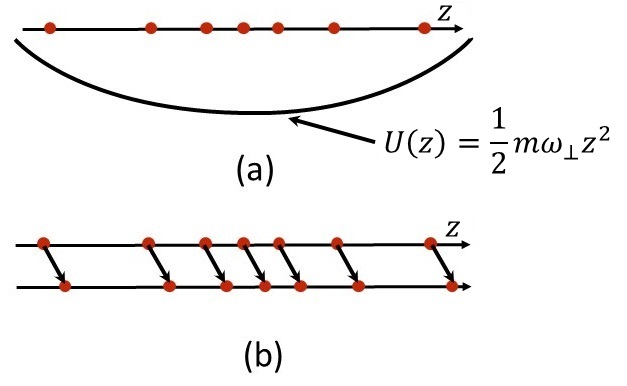
\includegraphics[width=0.7\columnwidth]{sloshing.jpg}
	\caption{Diagrammatic representation of the sloshing mode in a parabolic confinement:
	(a) particles trapped in a parabolic confinement.
	(b) when the system is suddenly shifted as a whole the whole system undergoes the sloshing oscillations with the same frequency $\omega_{\perp}$.\cite{Brey1989}}

	\label{sloshing}
\end{center}
\end{figure}


%MK REWRITTEN
\subsection{The Sloshing Mode}
\label{Sec:SM}
Let us consider a system of interacting particles on a $z$-axis, confined by a harmonic potential:
\be
U(z)=\frac{1}{2}m\omega_{\perp}^2z^2\, ,
\ee
which 
%Which 
subjects $\ell$th particle located at $z_{\ell}$ % away from the equilibrium position to a non-zero 
to a restoring force 
%MK of magnitude 
$m\omega_{\perp}^2z_{\ell}$ as shown in Fig.~\ref{sloshing}a. 
The particles are also subjected to a total interaction force exerted by all other particles.
%their neighboring particles. 
The condition for equilibrium for the system is that the net force acting on each individual particle has to be zero.
The equilibrium position of $\ell$th particle by $z^{(0)}_{\ell}$ are fixed by the requirement that the total force acting on each particle is zero,
\be\label{equil}
F_{\ell}=\sum_{\ell'\neq \ell}F^{int}(z^{(0)}_{\ell}-z^{(0)}_{\ell'})-m\omega_{\perp}^2 z^{(0)}_{\ell} =0\, ,
\ee
where $F^{int}(z_{\ell}-z_{\ell'})$ is the force experienced by the particle at $z_{\ell}$ due to the interaction with the other particle at $z_{\ell'}$.
It is crucial that this force is a function of the distance between the particles.

Away from equilibrium, $z_{\ell} \neq z_{\ell}^{(0)}$ the equations of motion, $m d^2 z_{\ell}/d t^2 = F_{\ell}$ have a sloshing solution,
\begin{align}\label{sl}
z_{\ell}(t) =  z^{(0)}_{\ell} + a \cos (\omega_{\perp} t)\, , \quad  \mathrm{for\, all}\, \ell.
\end{align}
Once all the particles are displaced by the same amount, $a$ off their equilibria, as shown in Fig.~\ref{sloshing}b, they keep sloshing collectively at frequency $\omega_{\perp}$ with no dissipation. 
Indeed, according to the equilibrium condition, Eq.~\eqref{equil} the force acting on the $\ell$th particle for a sloshing motion, Eq.~\eqref{sl} is the same as for particles without interactions,
\begin{align}
F_{\ell}(t)& =\sum_{\ell'\neq \ell}F^{int}(z^{(0)}_{\ell}+ a \cos (\omega_{\perp} t) -z^{(0)}_{\ell'}-a \cos (\omega_{\perp} t))-m\omega_{\perp}^2 (z^{(0)}_{\ell}  + a \cos (\omega_{\perp} t))
\notag \\
& = -m \omega_{\perp}^2 a \cos (\omega_{\perp} t)\, .
\end{align}
And since from Eq.~\eqref{sl}, $d^2 z_{\ell}(t)/d t^2 = - \omega_{\perp}^2 a \cos (\omega_{\perp} t)$, Eq.~\eqref{sl} solves the equations of motion.
%
%Now, if the entire system is suddenly shifted by an amount of $\Delta \bm{z}$, this gives rise to a non-zero net force on each particle.
%\begin{align}
%\bm{F}_i &=\sum_{j\neq i}\bm{F}^{int}(\bm{z}_i+\Delta \bm{z}-\bm{z}_j-\Delta \bm{z}) -
%m\omega_{\perp}^2(\bm{z}_i+\Delta \bm{z}) \notag \\
%&= -m\omega_{\perp}^2\Delta \bm{z}
%\end{align}
%The solution to the Newton's equation,
%\be
%m \ddot{z}_i = 
%\ee
%
% is %MK simply
%\be
%\bm{z}_i=\Delta \bm{z} \cos{(\omega_{\perp} t)}
%\ee
The obtained solution, Eq.~\eqref{sl} describes the particles oscillating collectively and in-phase with each other.
This is the sloshing oscillation mode. 
%MK Which means, all the particles oscillate with the same frequency which is equal to the characteristic frequency from the potential well. In other words, the entire system oscillates as a whole. 

The above discussion shows that the motion of each particle is unaffected by the interactions.
In what follows we explain how this result generalizes to the interacting Fermi liquid.
Interactions cause two effects, collisions and renormalization of different quasi-particle characteristics and thermodynamic quantities.
The inter-particle collisions do not disrupt the sloshing oscillations.
Indeed, similar to the above discussion, each small volume of the Fermi liquid moves as a whole without deformation.
Thanks to the Galilean invariance the energy of such a motion does not dissipate as heat by collisions.
More detailed discussion of the renormalization effects that parallels Sec.~\ref{Sec:SM} is given in Sec.~\ref{sec:Collective_spin}, 
where these effects are shown to cancel with the ``backflow'' contributions caused by the forces caused by the deviations from equilibrium.
Hence, at the moment to illustrate the idea we neglect interactions, and cast the previous arguments in terms of a kinetic theory. 
To this end, we find the sloshing oscillations as a solution to the Boltzmann transport equation.
%In this framework one studies the distribution function, $n_{\bm{p}}(\bm{r})$ in the six-dimensional phase space, $(\bm{r},\bm{p})$.

%MK LOTS OF CHANGES AROUND HERE

At equilibrium, $\mathfrak{n}_{\bm{p}}(\bm{r}) = n_F(\epsilon_{\bm{p}} + U(\bm{r}))$, where $n_F(x) = (e^{ (x - \mu)/T} +1)^{-1}$ is the Fermi-Dirac distribution function characterized by the temperature $T$ and the chemical potential, $\mu$.
The solution to the Boltzmann equation in this case 
\be\label{BE}
\partial_t \mathfrak{n} + \dot{\bm{p}}\cdot \bm{\nabla}_{\bm{p}} \mathfrak{n} + \dot{\bm{r}}\cdot \bm{\nabla}_{\bm{r}} \mathfrak{n} = 0\, , \quad
\dot{\bm{p}} = - \bm{\nabla}U(\bm{x}), \quad
\dot{\bm{x}} = \bm{v}_{\bm{p}}
\ee
can be obtained directly from the Liouville theorem. 
It reads, $\mathfrak{n}_{\bm{p}}(\bm{r},t)=n_F({\bm{r}}_{-t},\bm{p}_{-t})$, where $({\bm{r}}_{t},\bm{p}_{t})$ is the trajectory of a particle in the phase space obtained by solving the classical Hamilton equations of motion.
According to the discussion in Sec.~\ref{Sec:SM} we expect individual particles to oscillate around their equilibrium position.
Therefore we look for the solution of Eq.~\eqref{BE} in the form,
\be\label{try}
\mathfrak{n}= n_F[\epsilon_{\bm{p} + \hat{z} \alpha e^{i\omega t}} + U(\bm{r} + \hat{z} \beta e^{i\omega t}) ]\, .
\ee
It will suffice to solve Eq.~\eqref{BE} linearised in $\beta$ and $\alpha$.
Expanding the trial distribution function, Eq.~\eqref{try} in these quantities, one writes, $\mathfrak{n} = n_F + \mathfrak{n}'$, where,
\begin{align}\label{try1}
\mathfrak{n}'=
\partial_{\epsilon} n_F \left[ \bm{\nabla}_{\bm{p}}\epsilon_{\bm{p}} \cdot \hat{z} \alpha e^{i\omega t}  +  \bm{\nabla}U(\bm{r}) \cdot \hat{z} \beta e^{i\omega t} \right]\, .
\end{align}
We hence have to the linear order in $\beta$ and $\alpha$,
\be\label{BE2}
\bm{\nabla}_{\bm{p}} \mathfrak{n} = \partial_{\epsilon} n_F \hat{z} \frac{\alpha}{m} e^{i\omega t}\, ,\quad
\bm{\nabla}_{\bm{r}} \mathfrak{n} =  \partial_{\epsilon} n_F \hat{z} \beta k e^{i\omega t}
\ee
where the derivatives acting $\partial_{\epsilon} n_F$ may be omitted as any function of energy satisfies the Boltzmann equation identically thanks to the energy conservation.
The substitution of Eqs.~\eqref{try1} and \eqref{BE2} in Eq.~\eqref{BE} reduces the latter to two linear homogeneous equations,
\begin{align}\label{try2}
i \beta \omega -\frac{1}{m} \alpha =0\, , \quad %& = 0, 
%MK
%\notag \\
 k \beta + i \alpha  \omega = 0\, . %& 
\end{align}
%MK
The system, Eq.~\eqref{try2} have a non-trivial solution, $\beta,\alpha \neq 0$ only 
for $\omega= \sqrt{k/m}$ which is precisely %the sloshing mode frequency, 
$\omega_{\perp}$.

%MK
\section{Collective excitations in Bose superfluids}
The theoretical prediction of Bose-Einstein condensation have been around for almost a century, although the experimental realizations were made possible only after 1970s. Einstein, based on Bose statistics for photons \cite{Bose1924}, predicted that in a gas of massive, non-interacting bosons, below a certain temperature, a non-zero fraction of the particles would occupy the lowest energy single-particle state \cite{Einstein1924}. 

%In this part of the research we ask the following fundamental question.
%MKIt is known that 
% CHANGES
Superfluidity is the phenomenon that is distinct but interrelated to the Bose-Einstein condensation.
The capillary flow of the superfluid is %a 
meta-stable provided the flow velocity is below a certain threshold critical value, $v_c$.
In the extended system with the spectrum of elementary excitations $\epsilon_{p}$, $v_{c} = \min_p \{\epsilon_{p}/p\}$.
The flow in the narrow capillary tube dissipates into the topological vortex ring excitations.
For non-interacting particles, $\epsilon_p = p^2/2 m$, so that $v_c=0$ and such a system cannot be a superfluid.
Rather the superfluidity requires individual particles to lose their identity and form another, collective in nature excitations.
%MK
This process is expected to be efficient over a certain, so called healing length,  $\xi_h$ over which the particles are correlated.
Such correlations gives rise to a finite compressibility, which in turn, based on the general hydrodynamic considerations presented in 
Sec.~\ref{sec:sound_uniform} should result in sound waves.
Therefore, $\epsilon_p \approx v_s p$ for $p \lesssim \xi_h^{-1}$.
The transformation of the free particle dispersion, $\epsilon_p \approx p^2/ 2 m$ into a linear sound dispersion, $\epsilon_p \approx v_s p$ is the key mechanism linking the Bose-Einstein condensation and the superfluidity.

%, and $\epsilon_p \approx  p^2/2 m$ for $p \gtrsim \xi_h^{-1}$.
%In fact in the limit of weak interaction the Bogoliubov theory of superfluidity predicts, $\epsilon_p = \sqrt{p}$


%In the confined superfluid the motion is periodic with velocity that scales down with the amplitude of sloshing oscillations.
%At strictly zero temperature such oscillations do not dissipate below the critical velocity.

%and the question is whether it has a critical frequency below which it is protected from the dissipation.
%We will consider the weakly interacting Bose gas that undergo BEC transition.


%We start however from the non-interacting ideal gas with equation of state $p V = N T$ with the relation between the energy per unit volume and pressure $p = (2/3)\epsilon$.
%The full set of hydrodynamic equations in this case includes the continuity equation \eqref{cont}, Euler equation \eqref{Euler1} and the adiabatic transport condition, \eqref{s_cons} which we chose following \cite{Griffin1997} to write in the form \eqref{alt_s_cons2}.

%MK HAS TO BE REMOVED
%We write the linearized hydrodynamic equation in terms of the deviation of the particle density $\delta n = n - n_0(\bm{r})$  from the equilibrium density, $n_0(\bm{r})$, the velocity $\vec{v}$ and the deviation of the energy density $\delta \epsilon = \epsilon - \epsilon_0$  in the presence of the  confining potential $U(\vec{r})$. 
%These equations take form
%\begin{align}
%\frac{\partial \delta n}{\partial t} & = - \bm{\nabla} \cdot [ n_0(\vec{r}) \vec{v} ]
%\notag \\
%m n_0 (\vec{r}) \frac{\partial \bm{v}}{ \partial t} & = - \bm{ \nabla} P -  n(\vec{r},t) \bm{\nabla}U 
%\notag \\
% \frac{\partial \delta \epsilon}{\partial t } & = - \bm{\nabla} (\bm{v} \epsilon_0(\vec{r}))-  P_0(\vec{r}) \bm{\nabla} \cdot \bm{v} 
%\end{align}
%Using the equation $P = (2/3)\varepsilon$ and the condition of equilibrium,
%\be
%\nabla P_0 + n_0 \nabla U = 0
%\ee
%we rewrite the adiabatic transport condition in the form
%\be
% \frac{\partial P}{\partial t }  = - \frac{5}{3} \bm{\nabla} (\bm{v} P_0(\vec{r}))-  \frac{2}{3} n_0(\vec{r}) \vec{v}   \cdot \vec{\nabla} U
%\ee
%From these equation 
%\be
%m n_0(\vec{r}) \partial_t^2 \vec{v} = \frac{5}{3} \bm{\nabla} [\bm{\nabla}\cdot  (\bm{v} p_0(\vec{r}))] +  \frac{2}{3} \bm{\nabla}[ n_0(\vec{r}) \vec{v}   \cdot \vec{\nabla} U]
%+
%\bm{\nabla} \cdot [ n_0 \vec{v} ] \nabla U
%\ee
%For the one dimensional motion we get,
%\be
%\partial^2_t v = (5 k T/3 m)  \partial_x^2  v - \partial_x ( \omega_{\perp}^2 x v ) - (2/3) \omega_{\perp}^2 x  \partial_x v 
%\ee
%Look for the harmonic solutions,
%\be
%( - \omega^2  + \omega_{\perp}^2 ) v = (5 k T/3 m)  \partial_x^2  v  - (5/3) \omega_{\perp}^2 x  \partial_x v 
%\ee
%Rescaling the distances, 
%$x = y\sqrt{2 k T/ m \omega_{\perp}^2} $,
%\be
%(6/(5 \omega_{\perp}^2))( - \omega^2  + \omega_{\perp}^2 ) v =  \partial_y^2  v  -  2 y  \partial_y v 
%\ee
%The spectrum is therefore,
%\be
%v_n(y) = v_0 H_n (y)\, , \omega_n = \omega_{\perp} \sqrt{ ( 5 n + 3)/3}
%\ee
%$n = 0$ describes the Kohn mode.

%MK CHANGES
%\section{The Bose-Einstein condensates}

%MK MANY CHANGES IN THIS SECTION
\subsection{Dynamics of Bose condensate} %at zero temperature}
In a non-interacting Bose gas at $T=0$ all the particles occupy the same state.
Interactions cause a finite quantum depletion of this state as some particles are in states other than the non-interacting ground state.
If the interactions are weak the depletion is small and the description of the system in terms of a mean field becomes possible.
%In case of a weakly interacting Bose-Einstein condensate, practically all atoms occupy the same energy state. This enables the description of such systems in terms of a mean-field theory analogous to Hartree approximation. 
When the interaction are strong as is the case for liquid $\mathrm{^4He}$ the quantum depletion is significant and such an approach does not apply. 
%It must be noted that for strongly interacting systems like  this approach is inapplicable as there are strong correlations induced by the short-range interactions between atoms.


%First we wish to build 

We summarise the hydrodynamic formulation of Bose-Einstein condensates based on the 
%that describe the time-dependent behaviors of Bose-Einstein condensates. 
%We will start from the 
time dependent Gross-Pitaevskii equation\cite{Pethic}:
\be\label{tdGP}
i \hbar \frac{ \partial \psi(\bm{r},t) }{ \partial t } = -\frac{\hbar^2}{2m}\nabla^2\psi(\bm{r})+U(\bm{r})\psi(\bm{r})+V|\psi(\bm{r})|^2\psi(\bm{r})\, ,
%=\mu\psi(\bm{r})
\ee
%\be\label{GP}
%-\frac{\hbar^2}{2m}\nabla^2\psi(\bm{r})+U(\bm{r})\psi(\bm{r})+V|\psi(\bm{r})|^2\psi(\bm{r})=\mu\psi(\bm{r})
%\ee
where, $U$ is the external potential and $V_0$ is the effective low energy interaction amplitude.%energy in Gross-Pitaevskii approximation.
%MK , which is equal to the mean density of other Bosons around the atom at position $\bm{r}$ times the effective interaction. For a uniform Bose gas, the Gross-Pitaevskii equation is
For the uniform Bose gas the solutions with equilibrium, time independent density, $n_0 = |\psi(\bm{r})|^2$ have the form, 
$\psi(\bm{r},t) = \psi(\bm{r}) e^{ - i \mu t /\hbar}$, where the actual value of the density is fixed by Eq.~\eqref{tdGP},
$n_0 = \mu/V_0$.
%Just like the Schr\"odinger equation, this equation can also be written in a generalized time-dependent form:
%\be\label{tdGP}
%i\hbar\frac{\partial\psi(\bm{r},t)}{\partial t} == -\frac{\hbar^2}{2m}\delta^2\psi(\bm{r},t)+V(\bm{r})\psi(\bm{r},t)+U_0|\psi(\bm{r},t)|^2\psi(\bm{r},t)
%\ee
The basic Eq.~\eqref{tdGP} can be written in the hydrodynamic form.
In this formulation, the continuity equation has the same form, Eq.~\eqref{cont} as for the normal liquid, with
$\rho = m n = m |\psi|^2$.
The Euler equation, Eq.~\eqref{Euler1} is replaced by 
\be\label{Euler2}
m \frac{ \partial \bm{v}(\bm{r},t)}{\partial t} = - \bm{\nabla}\left[ U(\bm{r}) + n(\bm{r},t) V_0 - \frac{ \hbar^2 }{ 2 m \sqrt{n(\bm{r},t)} } \nabla^2 \sqrt{n(\bm{r},t)}  + \frac{1}{2}m v^2(\bm{r},t) \right],
\ee
where the flow velocity is $\bm{v} = (\hbar/m) \bm{\nabla} \phi$ with $e^{ i \phi} = \psi/|\psi|$.
In contrast to the normal fluid, the condensate flow is irrotational apart form the isolated singularities such as vortices.
As the condensate carries no entropy, the equation \eqref{s_cons} is trivially satisfied. 

The excitations spectrum is given by the dispersion relation of the small amplitude waves.
Considering the homogeneous liquid, $U=0$, we write as before, $n = n_0 + n'$ with $n' = n'_{\bm{q}}e^{ i \bm{q} \cdot \bm{r} - i \omega t}$.
As the flow is irrotational, we have $\bm{v} = \hat{q} v_q e^{ i \bm{q} \cdot \bm{r} - i \omega t}$ for $\hat{q} =\bm{q} /q$. 
To the linear order in $n'_{\bm{q}}$ and $v_{\bm{q}}$ Eqs.~\eqref{cont} and \eqref{Euler2} take form,
\begin{align}\label{l_GP}
\omega n'_{\bm{q}} - q n_0 v_{\bm{q}}& = 0\, ,
\notag \\
\frac{q}{m} \left(V_0 + \frac{ \hbar^2 }{ 4 m n_0 }  q^2 \right)n'_{q} -   \omega v_q & = 0\, .
\end{align}
The non-trivial solutions of Eq.~\eqref{l_GP} are obtained at the energies,
\begin{align}
\hbar \omega = \sqrt{ 2 n_0 V_0 ( \hbar^2 q^2 / 2 m ) + ( \hbar^2 q^2 / 2 m )^2}\, ,
\end{align}
As a result, in the long-wave length limit, $\hbar \omega = \hbar v_s q$, with the speed of sound,
$v_s = \sqrt{ n_0 V_0/m}$.
This result also follows from the relation, Eq.~\eqref{FL19} and the equilibrium condition, $ \mu = n_0 V_0$.
In the short-wave-length limit,   $\hbar \omega = \hbar^2 q^2/ 2 m$ describing the excitations of individual bosons.
The crossover between the wave-like and particle-like behaviour takes place for the wave-length of the order of the healing length,
$\hbar/(m v_s)$. 
The crossover scale is instrumental for the Thomas-Fermi approximation introduced in Sec.~\ref{sec:Bose}.
This approximation amounts to neglecting the term on the right-hand side of Eq.~\eqref{Euler2} that contains $\hbar$ explicitly.
For system size and the wave-lengths of the excitations exceeding the healing length the wave-like behavior dominates.

 


%Linearization of Eqs.~\eqref{cont} and \eqref{Euler2} around the equilibrium, $n = n_0$, $\bm{v}=0$ gives for the choice,  $n' = n'_{\bm{q}}e^{ i \bm{q} \cdot \bm{r}}$, 
 

%Now, we will derive the continuity equation for the particle density $n=|\psi|^2$, by multiplying \eqref{tdGP} by $\psi^*(\bm{r},t)$ and subtracting the complex conjugate:
%\be\label{BCcont}
%\frac{\partial n}{\partial t} + \bm{\nabla}\cdot(n\bm{v})=0
%\ee
%where, the velocity of the condensate is given by
%\be
%\bm{v}=\frac{\hbar}{2mi}\frac{(\psi^*\bm{\nabla}\psi-\psi\bm{\nabla}\psi^*)}{|\psi|^2}
%\ee
%and the momentum density,
%\be
%\bm{j}=\frac{\hbar}{2i}(\psi^*\bm{\nabla}\psi-\psi\bm{\nabla}\psi^*)
%\ee
%By expressing the wave function $\psi$ as a combination of an amplitude $f$ and a phase $\phi$ $(\psi=f\phi)$, we can see that the density depends only on the amplitude $(n=f^2)$ and the velocity depends only on the phase $(\bm{v}=\frac{\hbar}{m}\bm{\nabla}\psi)$. The equation of motion for $\phi$ provides us the necessary velocity equation:
%\be\label{BCveloc}
%m\frac{\partial v}{\partial v} = -\bm{\nabla}(\tilde{\mu}+\frac{1}{2}mv^2)
%\ee
%where, 
%\be
%\tilde{\mu}=V+nU_0-\frac{\hbar^2}{2m\sqrt{n}}\nabla^2\sqrt{n}
%\ee


%Now, we will linearize equations \eqref{BCcont} and \eqref{BCveloc} by considering small deviations from the equilibrium state of the condensate. We write the density as the sum of the equilibrium density and a small departure from the equilibrium: $n=n_{eq}+\delta n$. The linearized equations are:
%\be\label{BCcont-lin}
%\frac{\partial\delta n}{\partial t}=-\bm{\nabla}\cdot(n_{eq}\bm{v})
%\ee
%and
%\be\label{BCveloc-lin}
%m\frac{\partial\bm{v}}{\partial t}=-\bm{\nabla}\delta\tilde{\mu}
%\ee
%where $\delta\tilde{\mu}$ can be obtained by linearizing $\tilde{\mu}$. Combining equations \eqref{BCcont-lin} and \eqref{BCveloc-lin} provide us with the equation of motion for the system:
%\be
%m\frac{\partial^2\delta n}{\partial t^2}=\bm{\nabla}\cdot(n_{eq}\bm{\nabla}\delta\tilde{\mu})
%\ee
